%!TEX TS-program = xelatex
%!TEX root = ../../maxwell2018thesis.tex

\chapter[Models and Proposal]{Research Proposal and\\IIR Modelling}\label{chap:proposal}


% Previous chapters in this thesis discussed prior work that has been undertaken in the field of~\gls{acr:ir} -- and ~\gls{acr:iir}, with regards to stopping in search. In this chapter, we outline three key components that will be employed in the remainder of this thesis. In particular we will focus on:
%
% in this chapter, we will be proposing a new conceptual user model of search that advances the state of the art.
% then we will take heuristics, and formulate them into operational stopping strategies, that are formalised into rules that can be applied in practice. given chapters 5,6,7, we will empirically explore the quality of this model.
%
% We outline the main conceptual and theoretical contributions of this thesis, which is:
% - a more complex and realistic user model; and
% - enumerate the different stopping strategies that we will be evaluating.
%
% subsequent chapters are the empirical chapters, testing them out.
%
%
% less important:
% - method.
%
% ~~~~
%
% csm expl:
%
% updating the searcher model. considering the stopping
% paper at number 1
% focus at number 2
%
% main focus is on number 2.
% do some stuff with number 1.
% do some stuff with number 3.
%
% re-order the boxes.
%
% as outlined by maxwell and azzopardi, the reason why this has been brought in is because...
%
% **ad-hoc topic retrieval...could argue that the same basic process is followed for different search tasks, like navigational.
%
% we are focusing mainly on ad-hoc topic retrieval, because it facilitates the flow of this process many times.
% more interest to stopping strategies that people employ because they become more crucial.


\begin{itemize}
    \item[\emph{(i)}]{introducing an evolution of the conceptual user models of search, as previously discussed in Section~\ref{sec:stopping_background:models:conceptual};}
    \item[\emph{(ii)}]{discussing a number of different \emph{stopping strategies} that we will deploy within the revised model of search; and}
    \item[\emph{(ii)}]{provide a detailed overview of the general methodology that we will employ in subsequent contributory chapters of this thesis (Chapters~\ref{chap:temporal},~\ref{chap:snippets}, and~\ref{chap:diversity}).}
\end{itemize}

We begin this chapter by continuing along the same theme as what concluded the previous chapter: \emph{user modelling}. We introduce our revised model of the search process, the~\gls{acr:csm}.

\section{The Complex Searcher Model}\label{sec:proposal:csm}
The~\glsfirst{acr:csm} is a high level model of the search process, capturing the key stages undertaken by a searcher during the information seeking process. Illustrated in Figure~\ref{fig:csm}, the~\gls{acr:csm} is based upon prior models as proposed in the literature, previously discussed in Section~\ref{sec:stopping_background:models:conceptual}. Prime examples of prior models include the Markov-based approach by~\cite{baskaya2013behavioural_factors}, and the searcher model proposed by~\cite{thomas2014modelling_behaviour}. These models (along with others) are in broad agreement with the general sequence of events that searchers undertake during search, with searchers issuing queries, examining result summaries, and then examining documents for relevance. Refer to Figures~\ref{fig:baskaya_model_flow} and~\ref{fig:thomas_model} on pages~\pageref{fig:baskaya_model_flow} and~\pageref{fig:thomas_model} respectively for illustrations of the two aforementioned models.

Given the baselines outlined above and in Section~\ref{sec:stopping_background:models:conceptual}, the~\gls{acr:csm} offers a number of advancements of modelling the search process. These advancements are made in two key areas, both of which are discussed below.

\begin{itemize}
    \item{We provide improvements to the \blueboxbold{querying} aspects of the searcher model. Namely, a searcher subscribing to the~\gls{acr:csm} is able to generate an updated set of potential queries once he or she has completed interactions on a given~\gls{acr:serp}.}
    \item{We also introduce a \blueboxbold{further stopping decision point} concerning the \emph{overall impression} of a~\gls{acr:serp} once it has initially presented to the searcher.}
\end{itemize}

\noindent
\blueboxbold{Selecting a Query} With a search session an inherently interactive process~\citep{ingwersen2005theturn}, a searcher is able to \emph{learn} and develop their mental model of the given information need as they examine information presented to them. As such, during a search task, a searcher may decide to reformulate their query as they obtain a better appreciation of the topic, and are able to formulate a better query, perhaps with descriptive key terms. The~\gls{acr:csm} provides the mechanism for a searcher subscribing to such a model to update the list of potential queries that could be issued once he or she has finished examining a set of results from the previous~\gls{acr:serp}. This is in direct contrast to prior models of search, where queries were selected from a list generated at the start of the search session. This improvement in the modelling process permits a better representation of a searcher's so-called \emph{dynamic information needs}~\citep{borlund2003iir_model}.~\cite{maxwell2016agents} provide an in-depth discussion on this issue.

\begin{figure}[t!]
    \centering
    \resizebox{1\hsize}{!}{
    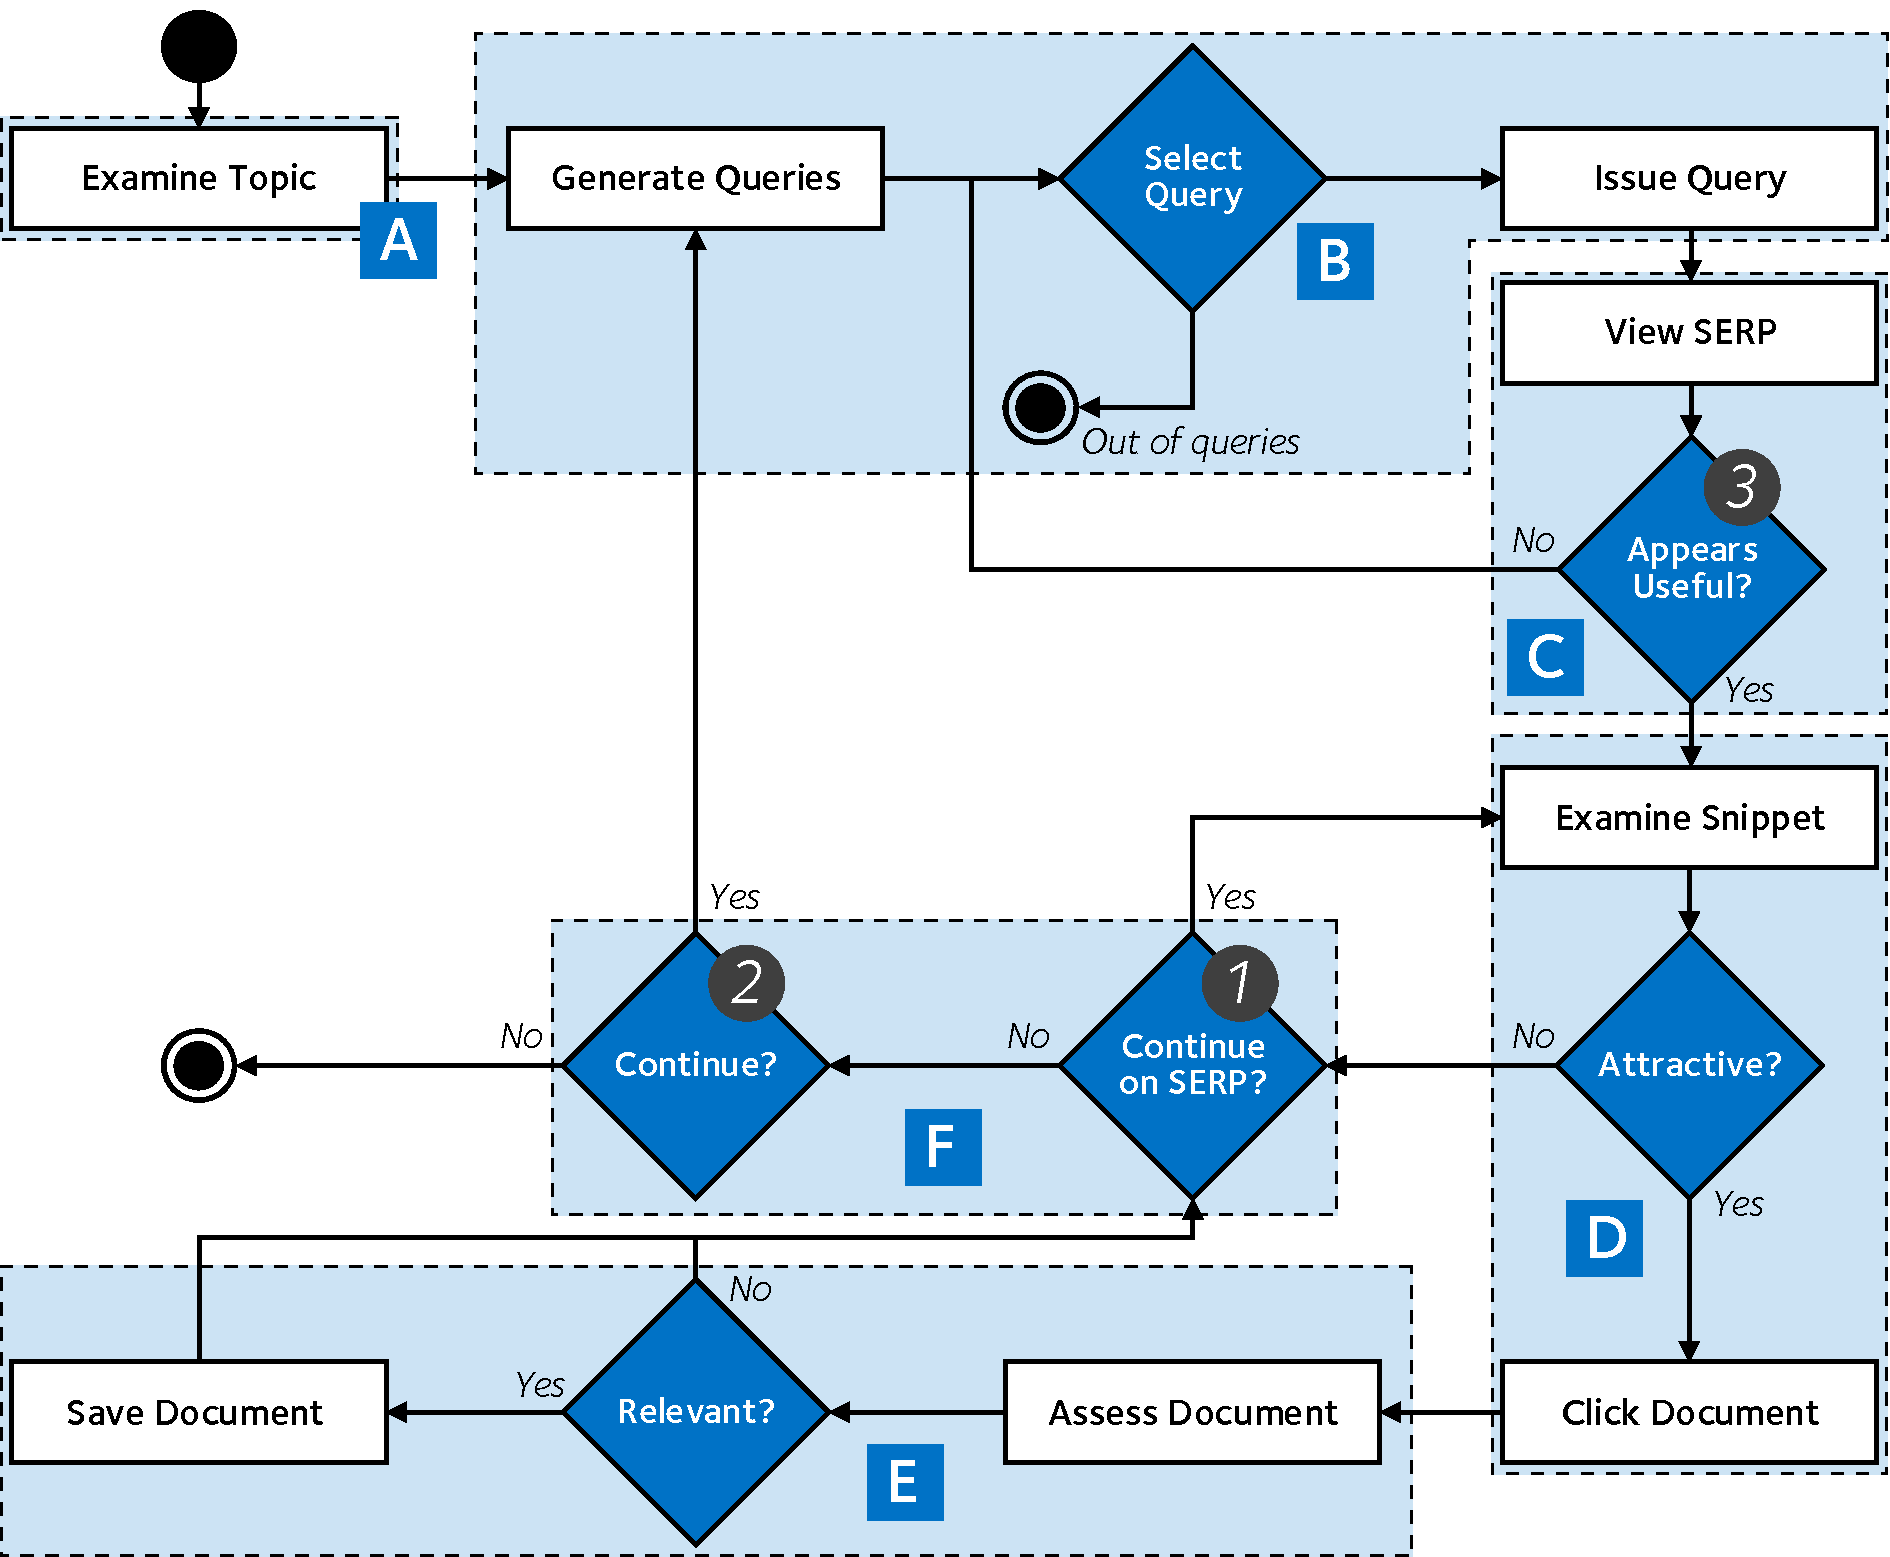
\includegraphics{figures/ch4-csm.pdf}}
    \caption[The Complex Searcher Model]{A flowchart of the proposed~\glsfirst{acr:csm}, as used in experimental work discussed later in this thesis. Refer to Section~\ref{sec:proposal:csm} for an explanation of each of the different components shown above. The three main \emph{stopping decision points} that the~\gls{acr:csm} considers – highlighted with \blueboxbold{1}, \blueboxbold{2} and \blueboxbold{3} – are discussed in Section~\ref{sec:proposal:model:stopping_points}.}
    \label{fig:csm}
\end{figure}

\noindent
\blueboxbold{New Stopping Decision Point} As mentioned above, the second development within the~\gls{acr:csm} is the inclusion of an additional \emph{stopping decision point} within the model. With two stopping decision points already present within established models of the search process (refer to Section~\ref{sec:stopping_background:models:conceptual:simple}), we propose a third -- the so-called \blueboxbold{\gls{acr:serp} stopping decision point}.

As outlined by~\cite{maxwell2018serp}, this additional stopping decision point is motivated by the idea of the \emph{information scent} present on a given~\gls{acr:serp}. This was briefly discussed in Sections~\ref{sec:stopping_background:user_studies:understanding} and~\ref{sec:stopping_background:models:theoretical:ift}, and in these sections we highlighted the concept of \emph{proximal cues} providing insights into whether the presented page will yield information that will aid the searcher in satisfying their underlying information need. This has been previously demonstrated in prior studies~\citep{wu2014information_scent, ong2017scent_behaviour, maxwell2017snippets}. By operationalising the notion of information scent as the perceived performance of a given~\gls{acr:serp}, we argue that incorporating this additional activity and stopping decision point allows a searcher to obtain an \emph{impression} of the~\gls{acr:serp} before deciding to \emph{enter} the~\gls{acr:serp} and examine content in detail, or \emph{abandon} the~\gls{acr:serp} and move to the next activity. In other words, when a poor query is issued, the searcher will not expend effort examining content which will have a high probability of not being relevant to their information need. The notion of forming an impression is similar to the summary impressions formed by searchers subscribing to the model defined by~\cite{thomas2014modelling_behaviour}, as detailed in Section~\ref{sec:stopping_background:models:conceptual:simple}. However, in this model, the searcher does not form an overview of the~\gls{acr:serp}, but rather an impression of each summary. This allows him or her to then deduce whether it is enticing enough to examine in more detail.

This is analogous to the well-studied phenomenon of \emph{\gls{acr:serp} abandonment} in which limited interaction occurs with the searcher. This has been typically assumed to provide an indication of the searcher's \emph{dissatisfaction} with the presented results~\citep{dassarma2008serp_abandonment, chuklin2012serp_abandonment}. Thus, we provide, to the best of our knowledge, a model of the search process incorporating a path for a searcher to abandon a~\gls{acr:serp} that appears to be of poor quality (or a \emph{low scent}).

\noindent
\blueboxbold{\gls{acr:csm} Assumptions} Of course, being a conceptual model of a real-world phenomenon, the~\gls{acr:csm} also makes a number of key assumptions, each of which are listed and detailed below.

\begin{itemize}
    
    \item{The~\gls{acr:csm} models the task of \blueboxbold{ad-hoc topic retrieval}, as previously discussed earlier in this thesis in Section~\ref{sec:ir_background:basics:cranfield:trec}. Numerous task types exist (e.g. patent search), and each task may vary slightly in terms of the order of activities -- and what activities are present.\footnote{This assumption is present at the request of Professor Nick Belkin, who discussed that this assumption should be made clear when the author of this thesis presented his work at the first \emph{ACM CHIIR} conference in Chapel Hill, NC, USA -- refer to~\cite{maxwell2016dc}.} Referring to Senior \emph{Microsoft} Applied Scientist Peter Bailey's \emph{SIGIR} paper tips\footnote{\url{https://www.microsoft.com/en-us/research/people/pbailey/} -- last accessed May 1\textsuperscript{st}, 2018.} -- specifically tip 10 -- we agree that ad-hoc topic retrieval is foundational to many areas of~\gls{acr:ir}, although it may not represent actual searcher behaviour in a real-world scenario, such as web search. According to Dr. Bailey, there is indeed \emph{``more to life than ad-hoc''}, though the scope of this thesis is generally restricted to such.}
    
    \item{The searcher, when subscribing to the~\gls{acr:csm}, is assumed to have already undertaken the necessary tasks to \blueboxbold{choose the search engine} that he or she will interact with. This is important to clarify, as models of search proposed in the literature -- such as the model by~\cite{thomas2014modelling_behaviour} -- assume a searcher decides what search engine to select, before beginning their interactions with it. Of course, this is an important step. For example, a patent searcher may use a bespoke search engine\footnote{For example, a patent searcher in the United Kingdom may utilise the \emph{Intellectual Property Office's} patent search engine, at \url{https://www.ipo.gov.uk/p-ipsum.htm} -- last accessed May 1\textsuperscript{st}, 2018.}, rather than a general purpose web search engine such as \emph{Google} or \emph{Bing}. We however consider this step superfluous to the requirements of the~\gls{acr:csm}.}
    
    \item{When considering whether the~\gls{acr:serp} should be abandoned, we assume that the searcher will always consider this decision under the pretence of \blueboxbold{bad abandonment} (i.e. a dissatisfaction of the presented results). This is in contrast to the notion of \emph{good abandonment}~\citep{khabsa2016good_abandonment}, which we do not consider within the~\gls{acr:csm}. Good abandonment is typically prevalent in contemporary search research (and on small-screen devices such as smartphones). With the inclusion of~\gls{acr:serp} components such as the information card~\citep{bota2016information_cards}, certain information needs can be satisfied by examining the~\gls{acr:serp} without needing to click on any results.}
    
    \item{For simplification, a~\gls{acr:serp} presented to a searcher utilising this model will consist only of one set of \emph{verticals}, i.e. the traditional \blueboxbold{ten blue links} that we still see today in contemporary search engines. However, contemporary web~\glsplural{acr:serp} also consist of additional components, such as the information card discussed above. Indeed, models have been proposed that incorporate additional~\gls{acr:serp} components, such as multimedia content in federated search~\citep{chen2012federated_search_click_model} (in this instance, a click model was derived). However, for simplification, the~\gls{acr:csm} assumes that such components are not present within a~\gls{acr:serp}.}
    
    \item{Once a searcher has decided to examine a~\gls{acr:serp} in detail, the result summaries presented to the searcher will be examined in \blueboxbold{linear order}. There is evidence to suggest that searchers in real life examine results from top to bottom, as demonstrated by~\cite{joachims2002click_model} and~\cite{joachims2005click_model}, for example. Click models, such as the \emph{cascade model}~\citep{craswell2008click_models}, have been developed that employ this assumption, where a searcher examines results in a linear fashion and stops once they have observed a relevant result. These approaches are all subject to \emph{positional bias,} that considers the notion that the searcher will trust the results of retrieval algorithm, and assume the first result is the most relevant.}
    
    \item{The~\gls{acr:csm} also assumes that the~\gls{acr:serp} presented to a searcher is \blueboxbold{not paginated.} This simplifies the modelling process somewhat, with pagination not included in searcher models previously examined in prior works, such as the TREC style user model (refer to Section~\ref{sec:stopping_background:models:conceptual:trec}).}
    
\end{itemize}

Combined together, these advancements demonstrate an improvement in user modelling, and should provide a more realistic means with which to model the process. While there are still assumptions in what is presented (i.e. no pagination) and how searchers interact with the~\gls{acr:serp} (i.e. examining results in a linear fashion), the improvements in the model should nevertheless lead to some improvements and provide a credible step forward in providing a better model of the search process.

\vspace*{5mm}
\begin{publications_box}{Associated Publications}
The~\gls{acr:csm} has been developed over a number years. Development of the model can be observed from a number of publications. The first version of the~\gls{acr:csm}, essentially analogous to the prior models of search outlined in Section~\ref{sec:stopping_background:models:conceptual:simple}, were outlined and used in simulated analyses, as reported in two publications.

\begin{itemize}
    \item{\bibentry{maxwell2015initial_stopping}}
    \item{\bibentry{maxwell2015stopping_strategies}}
\end{itemize}

Further developments to the~\gls{acr:csm} were found in a subsequent publication which experimented with the notion of \emph{intelligent search agents} (refer to \todo{Section~\ref{}}). Here, developments in the~\gls{acr:csm} led to the updating of the querying aspects of the model.

\begin{itemize}
    \item{\bibentry{maxwell2016agents}}
\end{itemize}

The final development of the~\gls{acr:csm} led to the inclusion of the third stopping decision point, complete with a large-scale simulated analysis. This led to the finding that the inclusion of the new decision point within the~\gls{acr:csm} led to improvements in overall search performance, and approximations of actual searcher behaviours.

\begin{itemize}
    \item{\bibentry{maxwell2018serp}}
\end{itemize}
\end{publications_box}

\subsection{Model Flow}\label{sec:proposal:csm:flow}
With the underlying assumptions and developments of the~\gls{acr:csm} now outlined, we next provide a high-level description of the various stages of the model. The~\gls{acr:csm} is illustrated as a flowchart in Figure~\ref{fig:csm} on page~\pageref{fig:csm}. Here, the model is described, with an explanation of the different processes involved, and the associated stopping decision points.

When subscribing to the~\gls{acr:csm}, a searcher, once he or she has attained a form of information need, will begin by performing an \blueboxbold{examination of the topic}. This is typically considered to be provided by an experimenter in the form of a \emph{TREC topic}, where a searcher will be provided with a predefined \emph{topic description} of what will constitute as a relevant document (refer to Figure~\ref{fig:topics} for examples). The searcher will then begin to formulate an initial mental model of the topic, identifying key terms and phrases that could be potentially used to translate this information need into a query formulation~\citep{borlund2003iir_model}.

\begin{figure}[t!]
    \centering
    \resizebox{1\hsize}{!}{
    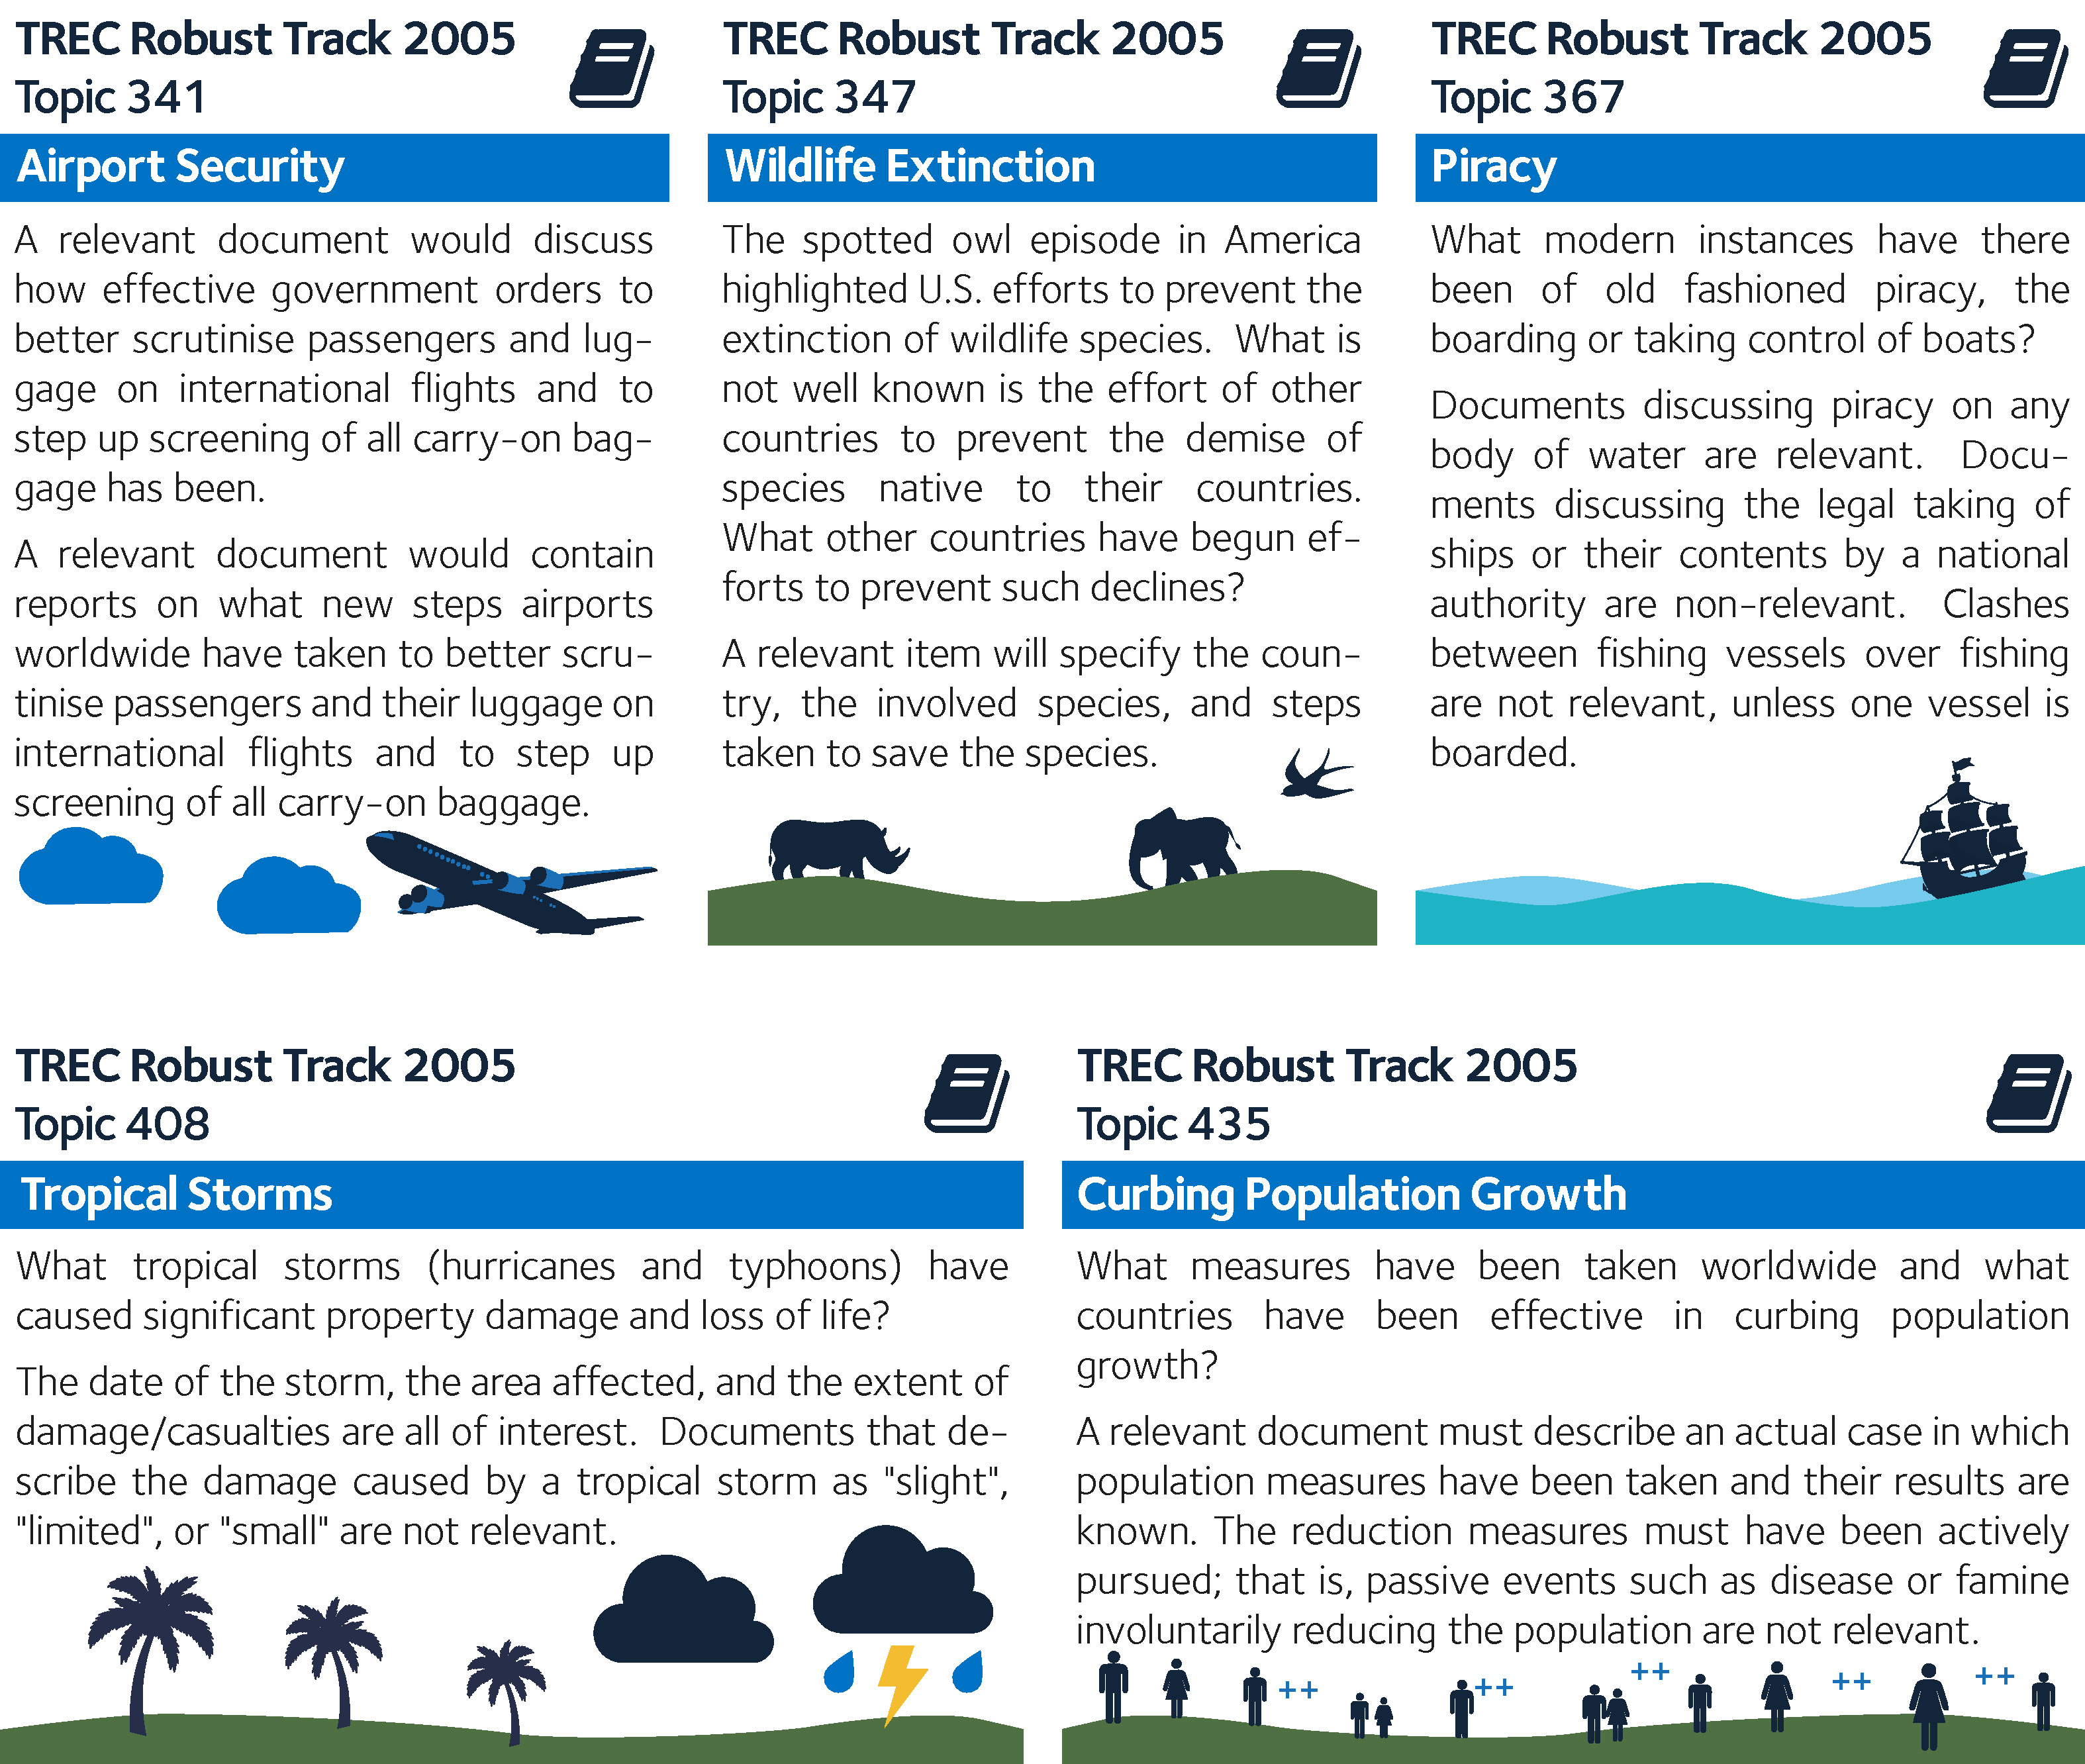
\includegraphics{figures/ch4-topics.pdf}}
    \caption[Examples of TREC Topics]{Three examples of \emph{TREC topic descriptions}, as outlined in Section~\ref{sec:proposal:csm:flow}. Topics are extracted from the \emph{TREC 2005 Robust Track,} as outlined by~\cite{voorhees2006trec_robust}. Descriptions provide an explanation as to what constitutes a relevant (and often non-relevant) document.}
    \label{fig:topics}
\end{figure}

Once a model of the information need has been established, the searcher will then move onto the \blueboxbold{query generation}, \blueboxbold{query selection} and \blueboxbold{query issuance} stages. Here, the searcher will employ some form of \emph{querying strategy} in order to formulate one or more queries from the underlying model of the information need, and then make a decision, \emph{selecting} one of the candidate queries to take forward and issue to the underlying search engine. It should be noted that if all candidate queries have been exhausted, the searcher will then stop their search session at this point. A number of \emph{querying strategies} have been proposed in the literature; refer to \todo{Section~\ref{}} for more information.

Once a query has been submitted the search engine, the searcher is then presented with the~\gls{acr:serp}. As per the assumptions stated earlier in Section~\ref{sec:proposal:csm}, we assume that the presented~\gls{acr:serp} consists solely of the result summaries -- including a title, snippet(s) and a document source for each. From here, the searcher is able to \blueboxbold{view the~\gls{acr:serp}} -- that is, obtain an \emph{initial impression} from examining the proximal cues presented to him or her. If the~\gls{acr:serp} does not appear to \emph{look good,} or offers a poor information scent, the searcher will abandon the~\gls{acr:serp} and proceed to then issue a further query from the list of candidate queries discussed previously.

If the~\gls{acr:serp} however appears to offer a high information scent, the searcher will then proceed to \blueboxbold{enter the~\gls{acr:serp}}. From here, individual \blueboxbold{snippets will be examined} in detail. As per the assumptions listed above, these are examined in a linear fashion. For each snippet, a judgement is made as to whether the searcher considers it to be sufficiently \blueboxbold{attractive} to click. If deemed sufficiently attractive, the link is clicked, and the searcher is then presented with the \blueboxbold{document} examined in full for an \blueboxbold{assessment}. Once complete, the searcher then makes a further decision with regards to the \blueboxbold{relevancy} of the document to the given information need (or topic, using~\gls{acr:trec} terminology). If deemed relevant, the document is then \blueboxbold{marked} as such, providing a simplistic means for determining what documents have been considered relevant and those that weren't -- refer to Section~\ref{sec:ir_background:user:evaluation:interactive_pr}.

Once the searcher has marked a document as relevant, he or she is returned to the~\gls{acr:serp}. At this point, the searcher must make a decision: \emph{should I continue to examine snippets on this current~\gls{acr:serp}?} This point is also reached by the searcher if he or she judges a snippet to have insufficient attractiveness to pursue further. If the answer is \emph{yes,} the next snippet is examined -- if the answer is \emph{no,} the searcher must then make a further decision. \emph{Given my overall search goals, have I met them? Should I continue my search session?} Search goals will vary between task type -- for ad-hoc retrieval, searchers will often attempt to find a predetermined number of relevant documents before a time limit expires. If the criteria have or criterion has not been met, the searcher will continue his or her search session by jumping back to the near start of the process, and undertake \blueboxbold{query generation} once more. If the stopping criteria have or criterion has been met, then the searcher will then abandon the search session, hopefully satisfied with what he or she has found.

Note that at each process -- whether it be issuing a query or examining a document for relevance -- a searcher will pay some form of \blueboxbold{cost} for the effort that they need to expend performing the aforementioned activity.

% \todo{Thursday -- start here.}
%
% Consider a chapter restucture:
%
% Part I: Introduction and Background
%     Intro
%     IR Background
%     IIR Stopping Background
%
% Part II: Modelling and Methodology
%     The Complex Searcher Model
%     Stopping Strategies
%     Methodology
%
% Part III: Stopping Behaviours
%     Time
%     Snippets
%     Diversity
%
% Part IV: Conclusions
%     Conclusion

\subsection{Stopping Decision Points}\label{sec:proposal:model:stopping_points}
Of central focus to the work in this thesis are the \emph{stopping decision points} of the~\gls{acr:csm}. As previously discussed, the~\gls{acr:csm} contains an additional, third stopping decision point. This is in combination with the two established stopping decision points, as previously highlighted in Section~\ref{sec:stopping_background:models:conceptual:simple} on page~\pageref{sec:stopping_background:models:conceptual:simple}.

The three stopping decision points that the~\gls{acr:csm} considers are listed below. While these are explained in Section~\ref{sec:proposal:csm:flow}, it is nevertheless good practice to enumerate them.

\begin{itemize}
    
    \item{\blueboxbold{\gls{acr:serp} Level Stopping} considers the point at which a searcher can abandon a~\gls{acr:serp} after attaining an \emph{initial impression} of the presented~\gls{acr:serp}, thus saving a searcher from examining summaries in depth if the~\gls{acr:serp} appears to be of poor quality.}
    
    \item{\blueboxbold{Snippet Level Stopping} As previously mentioned, this is sometimes labelled as \emph{query level stopping} in the literature. We name this decision point snippet level stopping to remove any ambiguity between~\gls{acr:serp} level stopping and this point. Snippet level stopping considers the depth to which a searcher will traverse a list of results, before deciding to stop their examination.}
    
    \item{\blueboxbold{Session Level Stopping} Finally, session level stopping concerns the notion of when a searcher will decide to terminate their search session altogether. This could be constrained by time limits, or some predetermined notion of how many relevant items they have found.}
    
\end{itemize}

Figure~\ref{fig:csm} on page~\pageref{fig:csm} also provides a visual illustration of the stopping decision points within the wider~\gls{acr:csm} flowchart. Decision points \blueboxbold{1}, \blueboxbold{2} and \blueboxbold{3} represent~\gls{acr:serp} level stopping, snippet level stopping and session level stopping respectively.

How these stopping decision points are operationalised is dependent upon a variety of different factors. For example, the task type is highly likely to influence the overall session stopping strategy that is employed. The literature, as overviewed in Section~\ref{sec:stopping_background:heuristics} provides a number of heuristics to potentially operationalise stopping. These are primarily geared towards the concept of snippet level stopping.

\subsection{Components of the Complex Searcher Model}
With the~\gls{acr:csm} high level and conceptual in nature, there are many different ways in which the model can be instantiated.


Of course, this model is high level and conceptual in nature. How can we instantiate it?
Being a high level, conceptual model, what are the main components, and how can they be instantiated?

What are the key components of the CSM, and what literature has been examined, in order to justify each of the blocks being present? Appendix~\ref{appx:simiir} provides an in-depth overview of the different components of the simulator framework used, which are essentially analogous to the blocks and decision points of the CSM.

\subsubsection{Topic Modelling}

\subsubsection{Query Formulation}

\subsubsection{SERP Abandonment}

\subsubsection{Decision Making}
The searcher has to make a number of decision points throughout the search process.
\emph{Is this relevant?}
Primarily stochastic in nature.

\subsubsection{Document Decision Making}
Information triage, basically a subset of decision making.

\subsubsection{Search Context}
what about a searcher's context?
remember what queries have been issued
remember what documents have been marked and examined, same for snippets.
leads on to the notion of \emph{state and agency.}

\subsection{Considering State and Agency}
- based upon probabilities of interaction
- but this is not the only way in which a user model can be instantiated.
- can develop autonomous agents in which the model is instantiated in such a way so that its decisions are deterministic, not stochastic.
- autonomous stuff is commonplace nowadays, recent example is the rocket launch.
- in search, autonomous agents were commonplace in the mid 2000's, with lots of research going into the exploration of search agency. (brief bit lifted from cikm 2016 paper).

- state is incorporated. indeed, we can argue that even the CSM I/II models consider state too -- but to a lesser degree. for example, the csm is able to consider what documents have been previously clicked on, or saved as useful.

- indeed, this was explored in detail, but is not provided in great depth here.
- refer to Appendix~\ref{appx:agency} for an analysis of incorporating state and agency within the CSM.

- however, this thesis focuses primarily on the notion of stochastic models of interaction, i.e. decision points are determined by the roll of a dice. this in itself introduces a number of additional issues that must be addressed (e.g. the law of averages) which are detailed in Section~\ref{sec:proposal:method:simulations}.

\section{Selected Stopping Strategies}\label{sec:proposal:strategies}
In Section~\ref{sec:stopping_background:heuristics}, we discussed a number of different \emph{stopping heuristics} that have been previously defined in the literature. A majority of these heuristics were derived from the concept of \emph{satiation}~\citep{simon1955satiation} -- that is, the searcher abandons their search when they feel satisfied with what they have found. These heuristics were conceptual in nature, being derived from a number of underlying theories and assumptions.

In this section, we take a number of these stopping heuristics forward to produce a number of different~\glsplural{glos:stopping_strategy}. These strategies are operationalised versions of the corresponding heuristics, which mean we can subsequently implement and test them. The stopping strategies are enumerated, and split into five main categories, as listed below:

\begin{itemize}
    \item{a baseline, \blueboxbold{fixed depth} stopping strategy;}
    \item{a stopping strategy based upon the \blueboxbold{frustration} stopping heuristic;}
    \item{\blueboxbold{satisfaction} based stopping strategies;}
    \item{a number of stopping strategies based upon the \blueboxbold{difference} threshold stopping heuristic; and}
    \item{several stopping strategies based upon~\blueboxbold{\gls{acr:ift}}.}
\end{itemize}

Note that these stopping strategies are primarily presented as snippet level stopping strategies -- they can in theory be applied to the other two stopping decision points of the~\gls{acr:csm}, as outlined previously in Section~\ref{sec:proposal:model:stopping_points}. We also do not consider every stopping heuristic mentioned previously in Section~\ref{sec:stopping_background:heuristics} -- a number of these heuristics, such as the mental list heuristic are not trivial to implement, and do not necessarily comply with the search task we will be simulating.

\noindent\blueboxbold{A Note on Usefulness} In this section, we refer to the concept of a result summary being \emph{useful} and \emph{unhelpful}. By this, we mean that a summary appears to be of use for a searcher to satisfy his or her information need. In the context of simulation, this notion of relevance does not necessarily correspond to the judgement made in a gold standard that is being compared to: the notion of usefulness in this context represents the decisions that are taken by a searcher as to what constitutes a useful or unhelpful document/result summary.

\vspace*{5mm}
\begin{publications_box}{Associated Publications}
Several of the stopping strategies listed in this section are based from previous work, listed earlier in this thesis.
\vspace*{-3mm}
\begin{itemize}
    \item{\bibentry{maxwell2015initial_stopping}}
    \item{\bibentry{maxwell2015stopping_strategies}}
\end{itemize}
\end{publications_box}

\subsection{Fixed Depth}
The fixed depth stopping strategy is based upon an assumption held across many of the models and measures that are widely used throughout the~\gls{acr:ir} community. This assumption is that a searcher, when examining a list of ranked results for their query, will browse to a \emph{fixed depth} before stopping -- the roots of which can be traced back to the Cranfield Paradigm as discussed in Section~\ref{chap:intro}. Examples of use include the basic stopping model encoded within~\gls{acr:patk}. The assumption is also widely used in the simulation of interaction. For example,~\cite{azzopardi2011economics} conducted a large-scale simulated analysis, where simulated users examined content to depths ranging from $5$ to $1,000$ ($1,000$ is typically assumed in TREC style experimentation, where a single query is issued). Given the wide use of this fixed depth approach in historical and contemporary~\gls{acr:ir} research, we consider this stopping strategy as the baseline approach to which we will be comparing the more advanced, \emph{adaptive} stopping strategies.

\begin{itemize}
    
    \item[]{\blueboxbold{SS1}} Using this stopping strategy, a searcher will stop once they have observed $x_1$ result summaries (i.e. \blueboxbold{SS1} @ $x_1$), regardless of their relevance to the given topic.
    
\end{itemize}

\begin{figure}[t!]
    \centering
    \resizebox{1\hsize}{!}{
    
\includegraphics{figures/ch4-ss1.pdf}}
    \caption[Examples of the fixed depth stopping strategy, \blueboxbold{SS1}]{An example of the fixed depth stopping strategy, stylised in this thesis as \blueboxbold{SS1}. Here, a searcher has an information need for the conference \emph{CIKM 2015} in Melbourne, Australia. The left example shows the top five results for poor performing query query, with few useful results (denoted by {\color{dmax_red}crosses}); conversely, the right shows results for a query performing well, with many useful results (denoted by {\color{dmax_green}ticks}). With \blueboxbold{SS1} @4, the searcher will stop at a depth of 4, regardless of the usefulness of the content provided.}
    \label{fig:ss1}
\end{figure}

Given the description of the stopping strategy above, we note that the fixed depth approach is na\"{i}ve in the sense that documents up to rank $x_1$ are useful to the searcher's given information need. On average, such a rule does make sense, but when individual result lists are considered, the approach would not be considered to be a sensible strategy to follow.

Despite the na\"{i}evty of the approach, the other main drawback of such an approach is exposed when a searcher complying with such a strategy issues a poor performing query. This is demonstrated in Figure~\ref{fig:ss1}, with two~\glsplural{acr:serp} presented side by side. Given a searcher's desire to find pages that provide information regarding \emph{CIKM 2015}\footnote{CIKM 2015 was a conference held in Melbourne, Australia, in October 2015. The paper that initially proposed many of these stopping strategies~\cite{maxwell2015stopping_strategies} was indeed presented at this conference.}, two queries are issued: the query on the left yielding poorer results than the query on the right, as denoted by the ticks and crosses, for useful and unhelpful result summaries, respectively. With \blueboxbold{SS1} @4 set, four result summaries are always examined before stopping, regardless of their perceived usefulness. As a result of this, na\"{i}vely examining four documents for the query on the left is by and large a waste of the searcher's time.

\subsection{Searcher Frustration}
The second category of stopping strategies that we propose in this thesis are those that consider a searcher's \emph{tolerance to non-relevance}. Given a set of result summaries presented on a~\gls{acr:serp}, how many would a searcher be prepared to judge to be of no use before they become frustrated, and subsequently abandon their query?

As detailed in Section~\ref{sec:stopping_background:heuristics}, a number of researchers have proposed stopping heuristics that consider non-usefulness (or \emph{non-relevance}, as defined in the literature). The rule intrinsically makes sense for exhaustive searches~\cite{kraft1979stopping_rules}. As an example, when tasked to find as many documents as possible related to different species of animals that are endangered, becoming disgusted with the presented~\gls{acr:serp} when a lack of new species are shown would be a suitable point at which to break and reformulate a new query, or abandon the search session altogether.

From the heuristics defined by~\citealt{cooper1973retrieval_effectiveness_ii} and~\citealt{kraft1979stopping_rules}, we propose two variants of the disgust rules, \blueboxbold{SS2} and \blueboxbold{SS3}.

\begin{itemize}
    
    \item[]{\blueboxbold{SS2}} Under this stopping strategy, the searcher will stop once they have observed $x_2$ unhelpful result summaries. If a result summary has been previously seen in the search session and was considered non-relevant, it is included in the count.
    
    \item[]{\blueboxbold{SS3}} Similar to the stopping strategy defined above above, a searcher employing this stopping strategy will stop once they have observed $x_3$ unhelpful result summaries \emph{in a row (contiguously)}. Previously observed unhelpful result summaries within the search session are included in the count.
    
\end{itemize}

\begin{figure}[t!]
    \centering
    \resizebox{1\hsize}{!}{
    
\includegraphics{figures/ch4-ss23.pdf}}
    \caption[Examples of frustration rules \blueboxbold{SS2} and \blueboxbold{SS3}]{An example of the two frustration rules, \blueboxbold{SS2} (left) and \blueboxbold{SS3} (right), both using a parameter of 3 unhelpful result summaries, and under the same query and results. Given that \blueboxbold{SS2} considers the \textbf{total} number of result summaries judged to be unhelpful, a searcher employing this stopping strategy would stop at rank 5 in the example above. Considering a set of contiguous unhelpful summaries, a searcher using \blueboxbold{SS3} would stop at rank 7.}
    \label{fig:ss23}
\end{figure}

As mentioned previously, these two stopping strategies are the first that we enumerate where a searcher would begin to \emph{adapt} their interactions with a ranked list of results, depending upon the performance of the underlying query that was issued. As such, this behaviour inherently makes these stopping strategies more realistic~\cite{moffat2013users_versus_models}. Figure~\ref{fig:ss23} illustrates this adaption in action, with the same query and associated results. On the left of the figure is an illustration of when a searcher employing \blueboxbold{SS2} would stop, and on the right, an example of \blueboxbold{SS3}. We use $x_2 = x_3 = 3$. Under \blueboxbold{SS2}, a searcher would stop at rank 5, while a searcher would stop at rank 7 when employing \blueboxbold{SS3}.

\cite{cooper1973retrieval_effectiveness_ii} highlights the above as one way of operationalising such a stopping strategy: by providing a pre-determined number of documents to stop at. The other approach, which we do not consider in this thesis, would be to allow a searcher to find a series of documents, then go back and count. Such an approach seems unnatural, with the former approach simulating a form of goal-based task. By varying the number of non-relevant documents to stop at, one will be able to attain a better understanding of how performance and other behaviours differ.

\subsection{Goal/Satisfaction Based}
Analogous to the frustration rule are the satiation-based stopping heuristics. Here, rather than focus on the frustration or disgust that a searcher might experience when confronted with unhelpful result summaries, satisfaction based rules -- explained in Section~\ref{sec:stopping_background:heuristics:judgement:satisfaction_frustration} -- consider a searcher encountering a number of \emph{useful} result summaries (or documents) before deciding to stop.

\begin{itemize}
    \item[\blueboxbold{SS4}] A searcher using this stopping strategy will stop examining content after encountering $x_4$ useful result summaries.
\end{itemize}

While demonstrated above in the context of snippet level stopping, such a strategy, depending upon the search task, may not be particularly useful when operationalised at this stopping decision point. For example, consider the scenario where a searcher issues a poor query, yielding next to no summaries deemed to be worthy of further examination. In this scenario, a searcher fully complying with \blueboxbold{SS4} may struggle to find enough documents to reach their goal, and this will waste time examining poor results. Such a stopping strategy may be better suited to an overall search goal (i.e. a session level stopping strategy), and deploying a more suitable stopping strategy for snippet level stopping decisions.

\subsection{Combination Rules}
Combination rule by~\citealt{kraft1979stopping_rules} that considers satiation and non-usefulness rules.

Combination rule that is defined in Foraging Theory.

\subsection{Considering the Difference}
Is something sufficiently different?


\begin{itemize}
    \item[\blueboxbold{SS5}] Term overlap difference
\end{itemize}

\begin{itemize}
    \item[\blueboxbold{SS6}] KL Divergence difference
\end{itemize}

\subsection{\glsfirst{acr:ift}}
This is foraging theory... when the rate of gain excee

\subsubsection{Optimal Foraging}

\begin{itemize}
    \item[\blueboxbold{SS7}] Optimal Foraging
\end{itemize}

\subsubsection{Time-Based Strategies}

\begin{itemize}
    \item[\blueboxbold{SS8}] Time-Based
\end{itemize}

\begin{itemize}
    \item[\blueboxbold{SS9}] Giving Up Rule
\end{itemize}

\begin{itemize}
    \item[\blueboxbold{SS10}] Combination of SS8 and SS9
\end{itemize}

\section{General Methodology Overview}\label{sec:proposal:method}

2 pages -- in the following chapters, this is what we are going to do.

ground the data
ground the simulation
evaluate it later on
explore influence of these decision points and stopping strategies under different contexts

We want to examine what happens to a searcher's behaviour when different stopping rules are employed under certain contexts.
How can we do this? Here, we provide a broad overview of the methodology that was employed in the later chapters of this thesis. Broadly split across two main sections.

Trial three different contexts to see what happens to searcher behaviour (in particular, stopping behaviour) when subjects to these contexts. In particular, what rules offer the best performance (and approximations)? Helps provide insights into the behavioural changes, and provides concrete evidence 

\subsection{Conducting a User Study}
- run the user study.
- collect the data using the treconomics framework.

\subsection{Extracting User Study Data}
- from the log file, ascertain key data points across the different experimental conditions or interfaces trialled.
- link back to the complex searcher model section to show where each of the probabilities and costs are used/employed.
- then, these costs can be fed into simulations, which can then be run (see Section~\ref{sec:proposal:method:simulations} below).

\subsection{Performing a Simulated Analysis}\label{sec:proposal:method:simulations}
Simulation as defined earlier is a good means for experimentation.
Low cost, always use the same users, no issue of learning bias, etc.

EXPLORE how people's behaviours change

- set up the probabilities
- instantiate the components

- pick a topic set
- pick a corpus
- basic structure of the methodology from previous papers

\subsection{Evaluating Performance and Approximations}
- how do we evaluate how good the system performs?
- how do we work out which one approximates best? on average.



\section{Chapter Summary}
In this chapter we have:

\begin{itemize}
    
    \item{Outlined the different stopping strategies we will employ}
    \item{Discussed the Complex Searcher Model (CSM) that will be used as the foundation to this work; and}
    \item{Provided a high level overview of the methodology that will be employed for the work central to this thesis.}
    
\end{itemize}